\chapter{Air Quality Monitoring System}

\section{Problem statement}

This section of the research depicts the problem statement of the project, which has encouraged us to go on with the project. According to research, the average annual PM 2.5 concentrations in Bangladesh were 77.1 microgrammes per cubic metre (mcg/m3) of air, which is seven times higher than the WHO exposure guidelines, with Dhaka standing second among 106 countries. Investigators from IQAir, a worldwide air quality information and technology enterprise, evaluated pollution data from 106 nations, specifically detecting PM2.5, a microscopic pollutant that can pose serious health concerns. 

To eliminate the climate change crisis, we have chosen a set of sensors with a microcontroller to detect the concentration of pollutants and monitor the data patterns. It will be turned to an IoT based device after the set of sensors are connected to the development board.

\vspace{0.5cm}
\section{System Analysis}
\vspace{0.5cm}

\vspace{0.5cm}
\subsection{4.2.1    Rich Picture AS IS}
\vspace{0.5cm}

\begin{figure} [H]
    \centering
    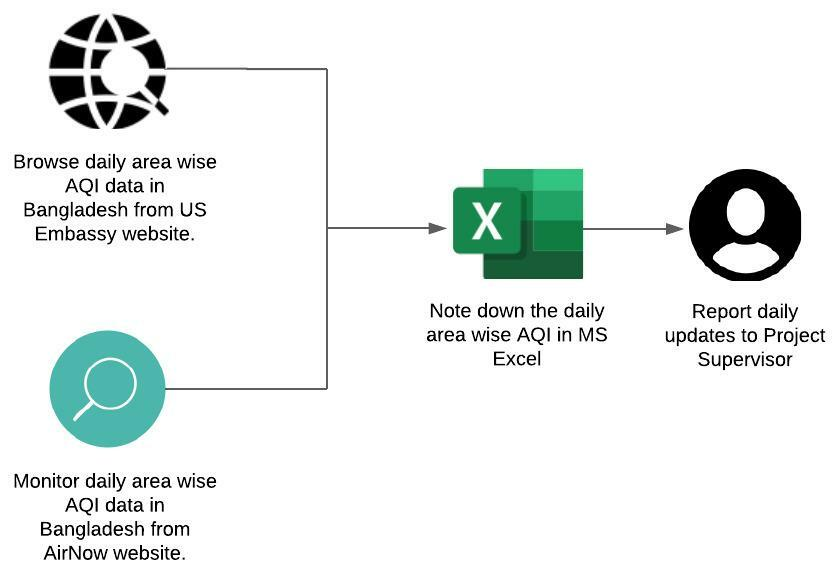
\includegraphics[width=.8\textwidth]{images/4_1_rich_pic_AS_IS.jpeg}
    \caption{Rich Picture AS IS}
    \label{fig:Rich Picture AS IS}
\end{figure}

\vspace{0.5cm}
\subsection{Six Element Analysis AS IS}
\vspace{0.5cm}




\vspace{0.5cm}
\subsection{Process Diagram AS IS}
\vspace{0.5cm}

\vspace{0.5cm}
\subsection{Problem Analysis}
\vspace{0.5cm}

\vspace{0.5cm}
\section{Proposed Solution}
\vspace{0.5cm}

We want to create an online web based big data driven solution which will help us monitor air quality and will help us make data driven decision making 

\vspace{0.5cm}
\subsection{Rich Picture TO BE}
\vspace{0.5cm}

\begin{figure} [H]
    \centering
    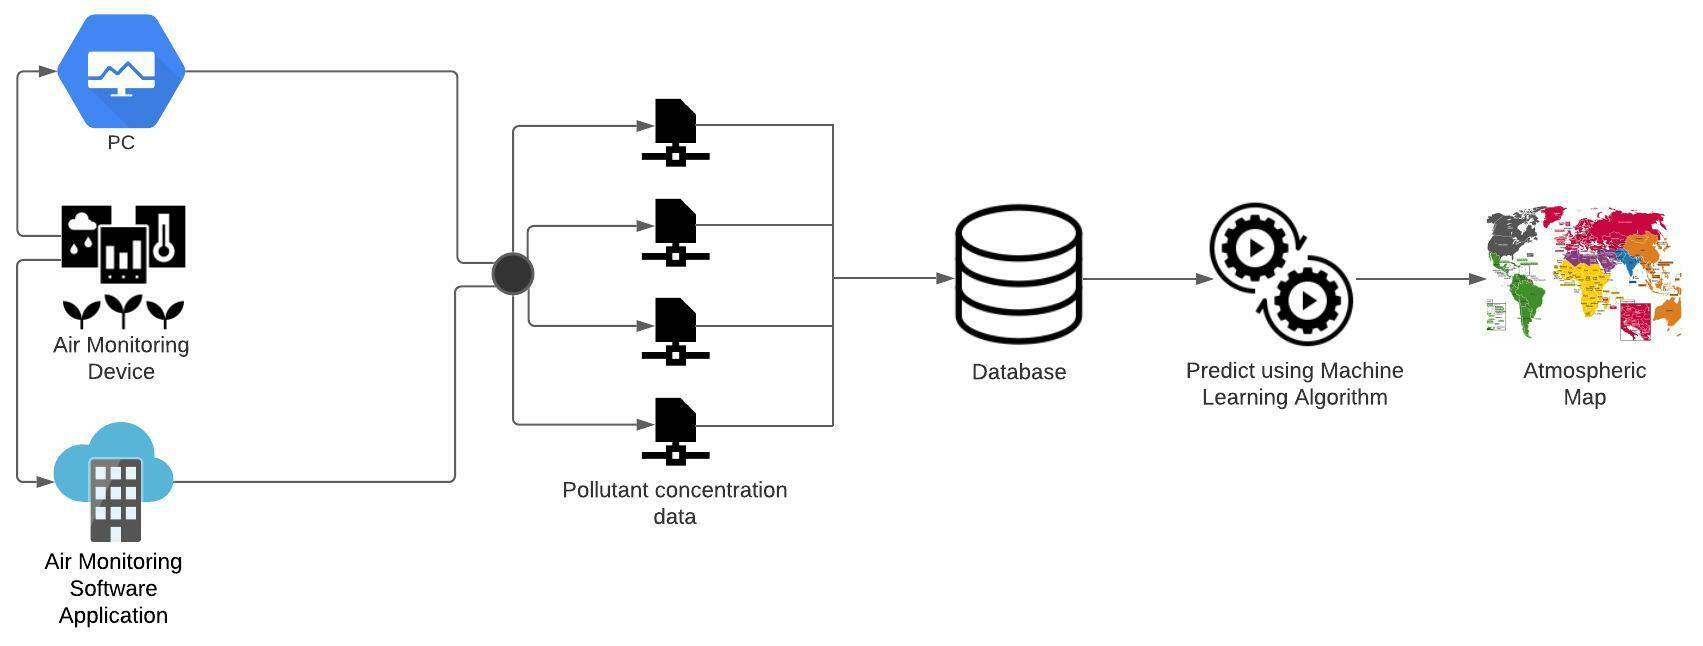
\includegraphics[width=.8\textwidth]{images/1_1_System Design AQM.jpeg}
    \caption{Rich Picture TO BE}
    \label{fig:Rich Picture TO BE}
\end{figure}

---------------
\subsection{UML Diagrams}
The activity diagram is an important UML diagram that shows the row of one activity to another. The activity diagram of the user and admin help to visualize the row of their activity in graphical form.

\begin{figure} [H]
    \centering
    \includegraphics[width=1\textwidth]{images/UML.jpg}
    \caption{ERP UML diagram}
    \label{fig:my_label}
\end{figure}

    



\subsection{Data Flow Diagram}Flow Chart Diagram: Describes the processes for the HP Chemical Factory I had analysed for: 


\begin{figure} [H]
    \hfill
    \includegraphics[width=1\textwidth]{images/HPCL - Editable-page-001.jpg}
    \caption{DFD part 1}
    \label{fig:my_label}
\end{figure}

\begin{figure} [H]
    \hfill
    \includegraphics[width=1\textwidth]{images/HPCL - Editable-page-002.jpg}
    \caption{DFD part 2}
    \label{fig:my_label}
\end{figure}   
\begin{figure} [H]
    \hfill
    \includegraphics[width=1\textwidth]{images/HPCL - Editable-page-003.jpg}
    \caption{DFD part 3}
    \label{fig:my_label}
\end{figure}
\begin{figure} [H]
    \hfill
    \includegraphics[width=1\textwidth]{images/HPCL - Editable-page-004.jpg}
    \caption{DFD part 4}
    \label{fig:my_label}
\end{figure}
\subsection{Use-case Diagram}
The use case diagram represents the functional requirements of the system. It shows the actors, cases, communication links, system and relationship.

\begin{figure} [H]
    \centering
    \includegraphics[width=1\textwidth]{images/Used Case Diagram.jpg}
    \caption{Used case Diagram}
    \label{fig:my_label}
\end{figure}
    
\subsection{Functional and Non-Functional Requirements}
\subsubsection{Functional Requirements:}

\begin{enumerate}

\item The authentication system validates the entered applicant’s name, email and unique password upon receiving the information and logs the user into the app by creating an account.
\item The system will generate unique ID for employees.
\item Verification of those provided information are done by sending a verification email to the applicant from the system. After which the applicant would be able to login.
\item The system will review if the inputted ID and password exists in the system or not.
\item The system will request for a password recovery if the ID is found but password is incorrect.
\item The system will request for new account if ID is not found in the system’s database.
\item The system will send a confirmation email to applicants after successfully creating accounts.
\item The system will let the employee choose different type of modules to work on.
\item The system will allow the applicants save their application to resume working on it later by clicking the button “Save Application”.
\item The application will only be submitted after the verification of payment for the form through Bkash or online banking.
\item The user’s personal dashboard must always be updated to show what information is missing and what they would need to do to complete their tasks. 
\item The system sends notification to the applicant when any updates are made.
\item The officers can search for the application by searching the username of the applicant or email.
\item The officers can also look up other officers to forward a task when required.
\item Admins will be able to add or remove employees in the system.
\item Admins will be able to update the template of the application form in the system and update policy when required in the system.
\item Geo-location based can record the applicant’s location as well as information like the number of applicants and the verified applications for the report.
\item The application will have customized sections to rearrange the dashboard form the default dashboard for each user to make it unique and more user friendly.

\end{enumerate}

\subsubsection{Non-functional requirements} 
\begin{enumerate}
\item Usability: The system is going to be user-friendly and aesthetically pleasing for the users.
\item Maintenance: This system/app is going to be maintained 2 times in a year, it runs smoothly and does not get slow or lag. Any bugs or problems can be fixed easily.
\item Valid data: All the information being updated in the system must be accurate and consistent for the users to take.
\item Scalability: The system can be accessed from any devices like: Computers, Smartphone’s. Apps for smart phones and an aesthetically similar web App for computers are developed.
\item Performance: Performance should always be smooth and easy to understand, such as searching and browsing for officers, submitting information and many more. These should leave a positive experience for users.
\item Service: Employees can use the system from all around the world. 
\item Reliability: The system will be backed-up for safety reasons and will not hamper and data during this process.
\item Control: As the system is initialized by the government, privacy will be maintained strictly. It will be completely secured and will be checked by the developer’s time to time for any sort of irregularity. 

\end{enumerate}
\section{Product Features}
Here I have included all the input and output features a user will receive from this project.
\subsection{Input}
\subsubsection{Login Page}
\begin{figure} [H]
    \centering
    \includegraphics[width=1\textwidth]{images/Login Page.JPG}
    \caption{Login Page}
    \label{fig:my_label}
\end{figure} 
\subsubsection{Sales Order Entry}
\begin{figure} [H]
    \centering
    \includegraphics[width=1\textwidth]{images/Create Order.JPG}
    \caption{Sales Order Entry}
    \label{fig:my_label}
\end{figure} 
\subsubsection{Complete Sales Order}
\begin{figure} [H]
    \centering
    \includegraphics[width=1\textwidth]{images/Sales Order Input.JPG}
    \caption{Complete Sales Order}
    \label{fig:my_label}
\end{figure}     
\subsection{Output}
\subsubsection{User dashboard}
\begin{figure} [H]
    \centering
    \includegraphics[width=1\textwidth]{images/Dashboard.JPG}
    \caption{User Dashboard}
    \label{fig:my_label}
\end{figure} 
\subsubsection{Delivery Process}
\begin{figure} [H]
    \centering
    \includegraphics[width=1\textwidth]{images/Putting the Shipment Number.JPG}
    \caption{Putting Shipment Number}
    \label{fig:my_label}
\end{figure}
\subsubsection{Complete Shipment}
\begin{figure} [H]
    \centering
    \includegraphics[width=1\textwidth]{images/Complete Shipment.JPG}
    \caption{Complete shipment}
    \label{fig:my_label}
\end{figure}    
\subsection{Architecture}

There are different types of architecture used in various systems. In our Oracle Fusion ERP system we used Three layers architecture for the client server \cite{chiu2003three}. 

\begin{figure} [H]
    \centering
    \includegraphics[width=.8\textwidth]{images/Architecture.jpg}
    \caption{three layers architecture for the client server}
    \label{fig:my_label}
\end{figure} 

